\documentclass{subfiles}

\begin{document}

    \chapter{Implementaciones sobre el sistema de Realidad Aumentada}
    \label{chap:3}

        \section{Modelo en 3D y Three.js}
        \label{sec:3.1}
        A partir del sistema básico generado en el capítulo anterior, podemos empezar a añadirle complejidad a nuestro sistema. El primer elemento que añadiremos es un modelo en 3D que utilizaremos como base en esta aplicación.

        \paragraph{}
        Para la carga, inserción, control y movimientos de los modelos en 3D se ha utilizado en esta aplicación la librería \threejs. \threejs es una librería ligera preparada para su uso en aplicaciones web compatible con \js \cite{web:wikipediathreejs}. Además, este está especializado en el control de modelos en 3D en formato \glb y \gltf, que son dos formatos basados en \textit{JSON} y que están creados para ser óptimos en tiempo de ejecución (el formato \glb es el equivalente en binario a \gltf) \cite{web:threejs_loading3dmodels}.

        \paragraph{}
        La librería \threejs basa su funcionalidad en el uso de Escenas o \textit{Scenes}, el objeto que utiliza esta librería para almacenar y presentar sus modelos en 3D, la iluminación o focos de luz que los alumbrarán y las cámaras virtuales que observarán a estos mismos \cite{web:threejs_scene}. Aplicando un símil sencillo, la Escena de \threejs podría equivaler a una escena de cine, donde los actores equivaldrían a los modelos en 3D, los focos equivaldrían a la iluminación y las cámaras equivaldrían a las cámaras virtuales. Este último concepto es muy importante, debido a que afectará continuamente al renderizado de los modelos en 3D.

        \paragraph{}
        La cámara virtual es la que simula el punto de vista del espectador, ya sea en \ra, en \rv o en otras virtualizaciones que utilicen modelos en 3D como son las simulaciones, los videojuegos o las películas de animación \cite{web:mozilla_virtualcamera}. A alto nivel, una cámara virtual, además de la posición del espectador, definiría también lo que este va a poder observar de manera que, cuando se va a renderizar una imagen, solo tiene que generarse la parte visible de los modelos que entren en el rango de visión de la cámara virtual.

        \begin{figure}
        \centering
        \fbox{
        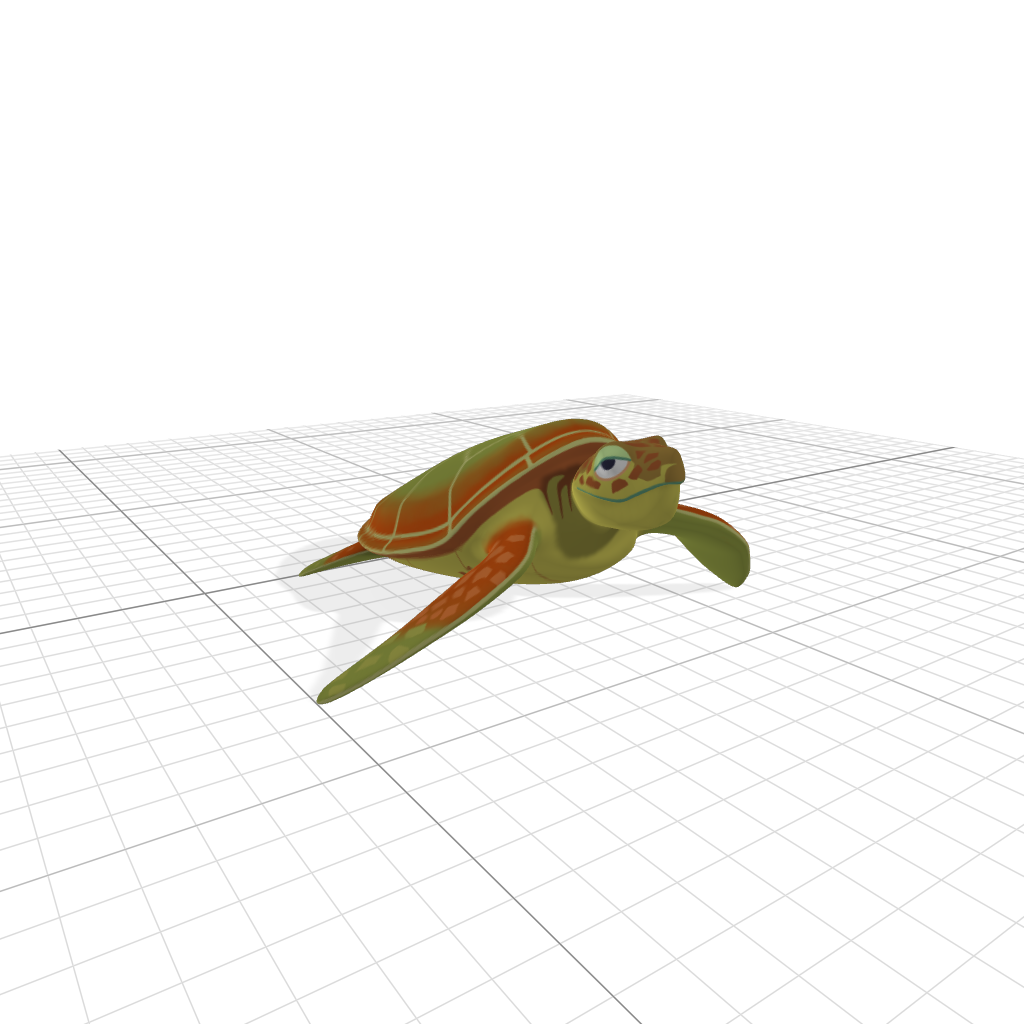
\includegraphics[width=0.6\textwidth]{img/tortuga_marina.png}
        }
        \caption{Ejemplo de renderizado de un modelo en 3D extraído de la biblioteca de modelos 3D de la aplicación de Windows \textit{Visor 3D}.}
        \label{fig:tortuga_marina}
        \end{figure}

        \paragraph{}
        Visualizando esto último con un ejemplo, en la figura \ref{fig:tortuga_marina} se ha renderizado un modelo 3D de una tortuga marina. En este renderizado, la cámara virtual se encuentra frente al modelo, pero ligeramente ladeado hacia la parte derecha de la tortuga. Debido a la posición de la cámara, no es necesario que se renderice la pata izquierda trasera de la figura, puesto que lo tapa el resto del cuerpo. Sin embargo, si la cámara se encontrase detrás de la tortuga, sería necesario renderizar ambas patas traseras y la cola, pero no se renderizaría la cara de la figura. De la misma manera, si la cámara no estuviese apuntando hacia la tortuga, no habría ningún modelo 3D que renderizar.
        
        \paragraph{}
        Aunque este parezca un concepto obvio, es necesario explicarlo, debido a que será necesario establecer la posición y orientación de la cámara virtual durante el desarrollo. Esto es porque la cámara virtual coincidirá con la posición de la cámara del dispositivo móvil. Cuando la cámara apunte hacia una figura en 3D en la \ra, se incrustará en la pantalla del móvil la parte de la figura que se vea desde la cámara virtual (es decir, se debe ver por la pantalla lo que se vería a través de la cámara si esta figura existiese en nuestra Realidad).

        \paragraph{}
        Una vez explicado esto, es necesario volver al código. Siguiendo el orden de carga, el primer lugar donde nos detendremos es en la función \textit{callback} \textit{checkSessionSupported}, vista en la sección \ref{sec:2.2}, que es la función que se lanza desde el constructor del Controlador y que inicializaba los elementos más pesados antes de que el usuario pulsase el botón de iniciar la Sesión de \ra. En esta, ya habíamos visto las acciones que se realizaban en caso de que el navegador no fuese compatible con \webxr, pero ahora vamos a ver algunas de las que se ejecutan en el caso positivo. Ampliando el código \ref{lst:2.2} al que hacemos mención:

\newpage
\begin{lstlisting}[language=JavaScript, caption={Carga de elementos de Three.js si se soporta la sesión.}, label={lst:3.1}]
// Constantes
#RETICLELINK = "http://url_donde_se_aloja_el_modelo_3d";

#checkSessionSupported = (isSupported) => {
    if (isSupported) {
    
        // Scene y Loader
        this.#scene = new THREE.Scene();
        this.#loader = new THREE.GLTFLoader();
        // ...

        // Modelo en 3D: Reticula
        this.#loader.load(this.#RETICLELINK, function(gltf) {
            // Figura
            this.#reticle = gltf.scene;
            this.#reticle.visible = false;
            this.#scene.add(this.#reticle);
        }.bind(this));
        // ...
    
    } else {
    
        document.getElementById("arButton").disabled = true;
        alert("Tu navegador no permite una sesi\xF3n de Realidad Aumentada.");
        
    }
};
\end{lstlisting}

        Aquí ya podemos ver tres elementos de cierto peso que se están cargando previamente antes de iniciar la Sesión: la Escena, una instancia de \textit{GLTFLoader} y, desde una función de esta última, un modelo 3D al que llamaremos a partir de ahora, <<retícula>>, sencillamente porque es el nombre del modelo original alojado en la librería de modelos de ejemplo de \webxr en GitHub. Este modelo en 3D, que podemos ver en la figura \ref{fig:reticle} será el que utilicemos como base para el funcionamiento de esta aplicación, haciendo las veces de <<puntero>> más adelante, cuando queramos señalar un punto en el suelo para ubicar la figura humana que desarrollemos.

        \begin{figure}
        \centering
        \fbox{
        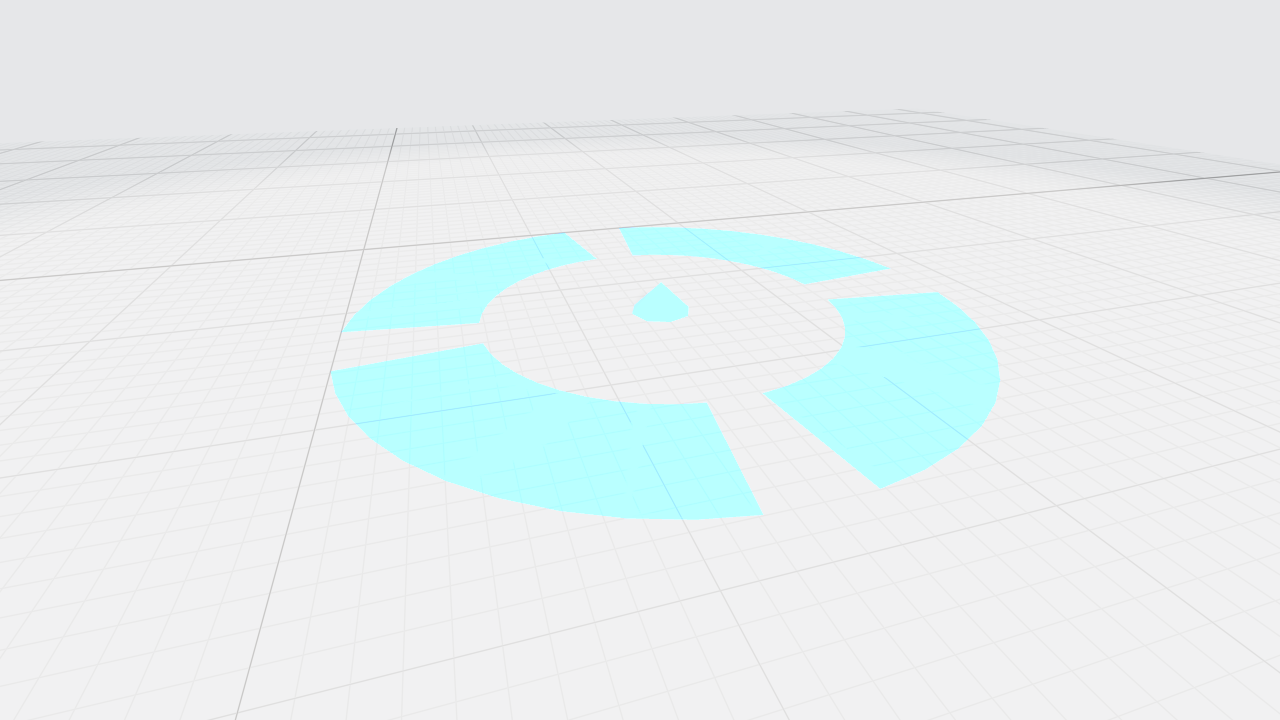
\includegraphics[width=0.6\textwidth]{img/reticle.png}
        }
        \caption{Muestra de la Retícula utilizada en esta aplicación. Modelo obtenido del repositorio \textit{webxr} del perfil de \textit{Immersive Web at W3C}, en GitHub.}
        \label{fig:reticle}
        \end{figure}

        \paragraph{}
        En primer lugar, inicializamos la Escena en la línea 8 para poder introducir la retícula más adelante (volviendo al símil anteriormente utilizado, es como si el actor <<retícula>> entrara en escena). Sin embargo, esto no lo podemos hacer hasta que se haya cargado el modelo. Para esto, utilizamos el objeto \textit{GLTFLoader} de \threejs \cite{web:threejs_gltfloader}, que es inicializado en la línea 9 para poder ser usado a continuación. Este objeto contiene la función \textit{load()}, que permite cargar un modelo 3D (en este caso, en formato \gltf o \glb, dado que este objeto es una especialización del objeto \textit{Loader} y solo permite cargar archivos de dichos formatos) y lanzar una función \textit{callback} una vez obtiene un resultado. Mediante la función de \textit{GLTFLoader}, \threejs hace la traducción del contenido del fichero a objetos de \threejs que sean manejables desde código. Aunque la documentación no sea muy extensa sobre el objeto que ofrece esta función, sí se puede encontrar que, mediante la función \textit{callback} que creemos para esto, recibiremos un objeto (que en la línea 13 hemos llamado \textit{gltf}) que contiene los siguientes atributos \cite{web:discoverthreejs}:

        \begin{itemize}
            \item \textit{animations}: devuelve un array con las animaciones (\textit{THREE.AnimationClip}) que contenga el archivo con el modelo 3D. Estas animaciones, aunque ya entraremos más en detalle más adelante, no son más que conjuntos de posturas que, agrupados de la manera correcta, dan la sensación de movimiento si se van recorriendo a una velocidad adecuada.
            \item \textit{scene}: aunque el sistema llame al atributo también <<Escena>>, en verdad el objeto contenido es de tipo \textit{THREE.Group}. Este objeto se puede definir como un conjunto de mallas de triángulos, que son los que formarán las superficies de los objetos tridimensionales. Al recoger todas las mallas del archivo de manera unida como un solo grupo, estaremos recogiendo en verdad el modelo 3D al completo.
            \item \textit{cameras}: en caso de que el archivo contenga una cámara virtual preestablecida, podremos encontrarlo en este atributo, que nos devolverá un array de objetos \textit{THREE.camera}. Estas cámaras no nos servirán para la \ra, porque nosotros queremos solamente una cámara que se encuentre en todo momento en el punto de vista de la cámara del dispositivo móvil. Este atributo es mucho más útil cuando se pretende utilizar la librería para aplicaciones web de visualización de este tipo de figuras tridimensionales, como pueda ser \textit{Babylon.js Sandbox}.
        \end{itemize}

        Estos son los atributos más importantes, aunque también contiene otros que son de menor importancia para el desarrollo hasta ahora de este proyecto: 

        \begin{itemize}
            \item \textit{asset}: objeto de \js sin tipo (\textit{Object}) que contiene metadatos del archivo, comúnmente generados de forma automática por la herramienta de diseño utilizada para la construcción del modelo.
            \item \textit{parser}: objeto \textit{GLTFParser} que contiene la información del objeto que se ha utilizado internamente para transformar el archivo.
            \item \textit{scenes} (no confundir con \textit{scene}): de manera similar a \textit{scene}, contiene un array de objetos de tipo \textit{THREE.Group}. Esto se debe a que los archivos \gltf pueden contener varios grupos separados de mallas, aunque no será el caso en este proyecto.
            \item \textit{userData}: objeto sin tipado que contiene información customizada por parte del creador del archivo. Esta no está estandarizada, por lo que la información podría estar de cualquier manera.
        \end{itemize}

        Como se puede comprobar, son muchos los elementos que se cargan de un solo archivo, aparte del propio modelo en 3D. Esto se debe a que, como se verá más adelante, al diseñar un modelo en 3D se pueden añadir distintas propiedades preestablecidas. Más adelante, en la sección \ref{sec:3.3}, veremos como, desde el mismo archivo del modelo, podremos acceder también a las animaciones predefinidas que se encuentren contenidas en este. Sin embargo, durante este diseño también se pueden preestablecer otros elementos y guardarlos en el mismo archivo como iluminaciones y cámaras virtuales.

        \paragraph{}
        Una vez sabemos esto, y volviendo al código \ref{lst:3.1}, podemos ver que, en la línea 15, se está almacenando en el atributo privado \textit{reticle} del Controlador el grupo de mallas que formarán el modelo 3D de la retícula. Después de esto, se establece la propiedad \textit{visible} de este modelo a \textit{false} para hacerlo invisible hasta que nos interese, y se añade (esta vez sí) a la Escena de nuestra \ra. De esta manera, ya tendremos la figura cargada y preparada para ser mostrada cuando sea necesario, teniendo en cuenta que todavía no se ha solicitado iniciar la Sesión de \ra.
        
        En el momento en que el usuario pulse el botón, 
        %% ubicacion de las figuras

        \section{Cálculo de superficies, \textit{Hit Test Results}}
        \label{sec:3.2}

        \section{Animación de modelos}
        \label{sec:3.3}
        %% clock
        %% comentar también el evento onTouch

        \section{Sonido espacial}
        \label{sec:3.4}
        %% comentar tambien el evento onsessionend

        \section{Funcionamiento final de la Realidad Aumentada}
        \label{sec:3.5}
        %% 
        %% carga aleatoria de figuras
        %% sustitucion de reticula por figuras

        

\end{document}